Having designed and implemented our gaze behaviors, we conducted a study with human participants, which aimed to answer the following research question: ``Can a virtual agent use its nonverbal cues---gaze and body orientation---to shape the footing of participants in multiparty interactions in a virtual environment?'' In our study, we had human participants engage in short, 10-minute conversations with a virtual agent and a simulated, avatar-embodied confederate. The participants would either experience the conversation on a 2D display or they would be immersed in the virtual environment using a VR headset (Oculus Rift). The virtual agent displayed gaze behaviors and body orientation shifts that would either include the participant as an addressee or exclude them as a bystander. Our primary goal was to show that the participant would conform to the conversational role signaled by the agent's footing cues---e.g., when assigned the role of a bystander, the participant would converse less with the agent. Our secondary goal was to show that these effects would be augmented in a virtual reality setting, where participants would have a better spatial awareness of their conversational partners' nonverbal cues.

\subsection{Hypotheses}

We designed a study to test the following hypotheses:

\begin{enumerate}
\item Participants will demonstrate conversational behavior that conforms to their footing as signaled by the agent's gaze and body orientation cues. Participants assigned the role of addressees will speak more. This is consistent with research on human conversational behavior, which shows that conversing partners tend to orient themselves in an particular arrangement called F-formation~\citep{kendon1990conducting} and that people tend to look at the addressees of their utterances~\citep{kendon1967some}.
\item Participants will evaluate the agent more positively if they are assigned the role of addressees rather than bystanders. This is consistent with findings that people who make a lot of eye contact are viewed as more likeable and credible~\citep{argyle1976gaze,beebe1976effects}.
\item Participants will feel more groupness and closeness to the agent if they are assigned the role of addressees, because reduced gaze toward bystanders will lead to feelings of ostracism and exclusion~\citep{wirth2010eye}.
\item The agent's footing cues will have a stronger effect on the participants' conversational behavior (Hypothesis 1) in the VR setting than when using a 2D display.
\item The agent's footing cues will have a stronger effect on the participants' subjective perceptions of the agent (Hypothesis 2) in the VR setting than when using a 2D display.
\item The agent's footing cues will have a stronger effect on the participants' feelings of groupness and closeness (Hypothesis 3) in the VR setting than when using a 2D display.
\end{enumerate}

Hypotheses 4-6 are motivated by the fact that the use of immersive VR brings about heightened awareness of the agent's nonverbal cues, partly because it blocks out external visual stimuli, but also because the Rift's high field of view (110$^\circ$) affords a much better view of the agent, confederate, and environment than what is possible on a 2D screen. Furthermore, the head tracking capabilities allow more intuitive control over the viewpoint than the traditional mouse-look interface, making it quicker for the participant to reorient their viewpoint toward the agent when the latter says or does something important.

\subsection{Design}

The study followed a mixed, 2x2 factorial design. The independent variables were \emph{agent behavior} and \emph{task setting}. The agent behavior variable was between-participants and had the following levels:

\begin{enumerate}
\item \emph{Exclusive} -- The agent displayed nonverbal behaviors that would exclude the participant from the interaction as a bystander. It would orient its body toward the confederate (facing them straight-on) and gaze at them much more than at the participant, in accordance with the distributions given in Table~\ref{tab:GazeFootingSpatial}.
\item \emph{Inclusive} -- The agent displayed nonverbal behaviors that would include the participant in the interaction as an addressee. It would distribute its body orientation evenly between the participant and the confederate (using the mechanism depicted in Figure~\ref{fig:FTorsoAlign}, and gaze at them equally (Table~\ref{tab:GazeFootingSpatial}).
\end{enumerate}

\begin{figure}
\centering
\includegraphics[width=1\textwidth]{conversationalrolegaze/Figures/GazeFootingConditions.pdf}
\caption{Diagram illustrating the conditions of the agent behavior independent variable. Upper row: conversational formation. Bottom row: participant's view of the scene.}
\label{fig:GazeFootingConditions}
\end{figure}

Figure~\ref{fig:GazeFootingConditions} illustrates the agent behavior manipulation. The upper row of images show the conversational formations resulting from agent's body orientation shifts at each level of the manipulation, whereas the bottom images show the views of the scene from the participant's perspective.

The other independent variable, task setting, had the following levels:

\begin{enumerate}
\item \emph{2D display} -- The participant experienced the interaction on a 27'' Dell monitor, at 2560x1440 resolution and a field of view of 50$^\circ$, while using the mouse to control the viewpoint.
\item \emph{VR} -- The participant wore a VR headset (Oculus Rift CV1). They saw the scene at the resolution of 1080x1200 per eye, with a 110$^\circ$ field of view. Built-in head orientation tracking and the external positional tracker allowed the participant to control the viewpoint by moving their head.
\end{enumerate}

The screenshots in Figure~\ref{fig:GazeFootingConditions} are both from the \emph{2D display} condition. The use of the Oculus Rift in the \emph{VR} condition afforded a much higher field of view and more natural control over the viewpoint, allowing the participant to easily see both the agent and the confederate simultaneously, as well as shift their gaze from one to the other by simply moving their head.

Since the study had a within-participants factor, we implemented two versions of the task to minimize transfer effects. The tasks were identical in structure and duration, and they had similar content. The participants were assigned to conditions in a stratified order, counterbalanced with respect to task setting (\emph{2D display} or \emph{VR}) and task version (\emph{Task 1} or \emph{Task 2}).

\subsection{Task}

\begin{figure}
\centering
\includegraphics[width=1\textwidth]{conversationalrolegaze/Figures/GazeFootingTask.pdf}
\caption{Left: the participant's view of the scene at the start of the task. Right: physical task setup.}
\label{fig:GazeFootingTask}
\end{figure}

The study task was a three-party interaction in a virtual room. The interaction took the form of a casual, interview-style conversation moderated by the agent. The conversational partners were the agent, the participant, and a simulated, avatar-embodied confederate. At the start of the task, the participant would find themselves standing at the room's entrance with a view of the agent and confederate on the other side of the room (Figure~\ref{fig:GazeFootingTask}, left); the agent and confederate would face each other in a vis-a-vis formation. The participant was prompted to click a button (either on the mouse or the Oculus Remote) to initiate the interaction; upon doing so, the camera would automatically approach the agent. Depending on the agent behavior condition, the agent would either glance at the participant and continue facing the confederate (\emph{exclusive} agent behavior) or reorient herself toward the participant (\emph{inclusive} agent behavior).

After introducing herself and greeting the partners, the agent would begin asking casual questions about their life experiences and interests. Some questions were designed to elicit short, one-sentence responses (e.g., ``What is your favorite movie?''), while others elicited longer, more open-ended responses (e.g., ``What is your favorite movie about?'') Most questions were implicitly addressed at both the participant and confederate, and they both had a choice in answering them. Our expectation was that the participant was more likely to take the conversational floor and answer the question if the agent demonstrated more inclusive nonverbal behaviors. A speech recognition system was used to detect when the participant was speaking. While the participant was speaking, the agent would look at them.

The confederate was simulated and its behavior was scripted. At the end of the agent's turn, the system would randomly decide if the confederate should answer the current question or not. If yes, the confederate would take the floor within about 0.75 $s$ and give a prerecorded response to the question. If not, the system would wait up to 3.4 $s$ for someone to speak out; if no one did, either the confederate would take the floor and answer, or the agent would proceed with the next question. The pause values between turns are derived from measurements of human speech in prior work and padded for possible speech recognition lag. According to~\citet{weilhammer2003durational}, the mean pause between turns is about 380 $ms$ in spontaneous American-English discourse, whereas silences longer than 3 $s$ are experienced as uncomfortable~\citep{mclaughlin1982awkward}.

\subsubsection{Setup}

The physical setup of the task is shown in Figure~\ref{fig:GazeFootingTask}, right. Participants were seated in an office chair in front of a personal computer while wearing an audio headset (in the \emph{2D display} condition) or Oculus Rift (in the \emph{VR} condition). A video camera was set up to record their behavior.

\subsubsection{Implementation}

The task was implemented in Unity game engine. The task logic, the agent's conversational behaviors, and task measurements were all implemented in C\# scripts. Microsoft Speech SDK was used for speech detection and the agent's speech synthesis and lip-sync, while Oculus Lip Sync was used to animate the confederate's lip movements. The agent and confederate character models were imported from DAZ. Both models had a looping, idle body animation applied to enhance the naturalness of their behavior.

\subsection{Participants}

We recruited 32 participants (17 female and 15 male) through an online student job website as well as in-person recruitment. All the participants were students. 27 participants were native English speakers.

\subsection{Procedure}

We conducted the experiment in a small, closed study room with a computer table. The participants were ushered into the room by the experimenter and seated at the table. Following a brief overview of the task, they were given a consent form to read and sign. Next, they were given detailed task instructions and handed an instructions sheet to serve as a reminder. The experimenter would then launch the task application and leave the room. Upon task completion, the participants were handed a questionnaire for subjective evaluation of the agent and task. This was followed by a second trial of the task, upon which the participants would fill out another subjective questionnaire and a brief demographics questionnaire. Finally, the participant received payment in the amount of \$5. Total experiment duration was 30 minutes.

\subsection{Measures}

The experiment involved two behavioral and several subjective measures. The behavioral measures were designed to measure the participants' level of participation in the interaction, in order to test Hypothesis 1. They were the following:

\begin{enumerate}
\item \emph{Number of speaking turns} -- Total number of speaking turns taken by the participant over the course of the interaction.
\item \emph{Total speaking time} -- Cumulative length (in seconds) of the participant's speaking utterances over the course of the interaction.
\end{enumerate}

When calculating the behavioral measures, we excluded participants' responses to the first five questions (out of twenty-five total) to allow for acclimation.

The subjective measures were collected using the subjective questionnaire and consisted of seven-point scale items. The measures were the following:

\begin{enumerate}
\item To measure the agent's likeability, we had participants rate the agent on traits such as likeability, cuteness, and friendliness. From this data we constructed a scale consisting of two factors: \emph{likeability} (two items, Cronbach's $\alpha = 0.824$) and \emph{attractiveness} (three items, Cronbach's $\alpha = 0.929$).
\item Feelings of \emph{closeness} to the agent were measured using a four-item scale (Cronbach's $\alpha = 0.823$) adapted from~\citep{aron1992inclusion}, which had participants indicate their agreement with statements such as: ``The agent paid attention to me.''
\item Groupness was measured using a scale adapted from~\citep{williams2000cyberostracism}, which consisted of seven items (Cronbach's $\alpha = 0.827$) and had participants indicate their agreement with statements such as: ``I felt ignored or excluded by the group.''
\end{enumerate}

Our questionnaire also included two checks for the agent behavior manipulation (also seven-point items): (1) ``The agent faced me during the interaction'' and (2) ``The agent faced the other participant.''

\subsection{Results}

Having collected our data, we first performed an analysis of variance (ANOVA) on the manipulation checks. We found no significant effects of the agent behavior manipulation on either check, $F(1, 61) = 1.931, p = .170$ and $F(1, 62) = 2.703, p = .105$. We believe this is due to ambiguous wording of the questions, as well as the use of a seven-point scale. It may not have been clear to our participants if ``facing'' referred to body facing or the amount of gaze. In either case, there is no clear mapping from a seven-point scale to either of these quantities, which is likely to have contributed to the ambiguous and noisy check results.

Additionally, we confirmed that \emph{task version} had no significant effect on any of our behavioral or subjective measures, suggesting the two tasks were sufficiently similar for our purposes.

\subsubsection{Behavioral}

\begin{figure}
\centering
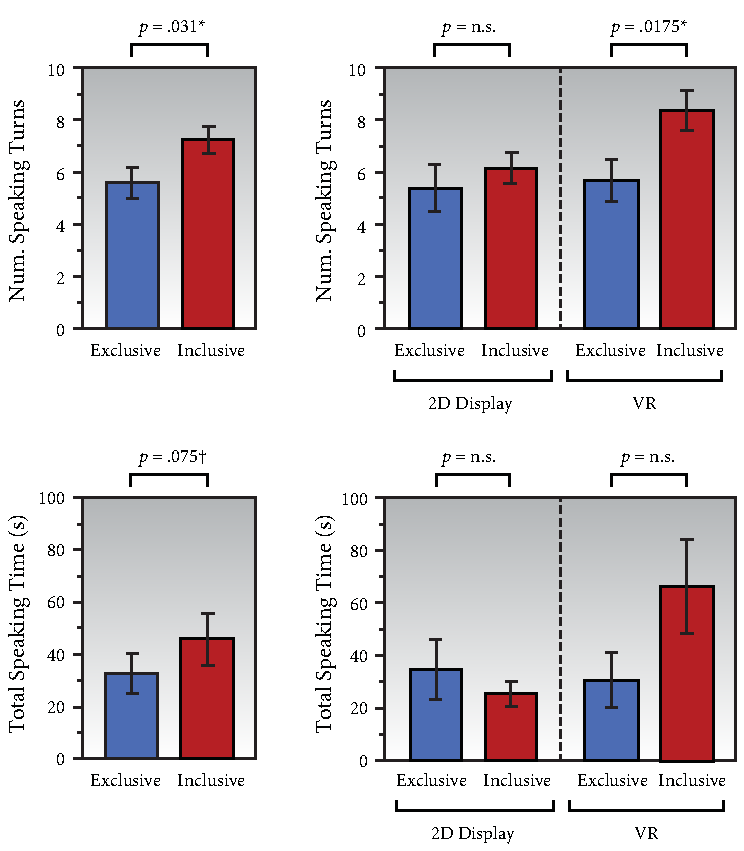
\includegraphics[width=0.95\textwidth]{conversationalrolegaze/Figures/ResultsBehavioral.pdf}
\caption{Results from behavioral measures. Left: number of speaking turns (top) and total speaking time (bottom) by agent behavior (\emph{exclusive} vs. \emph{inclusive}). Right: same measures by agent behavior and task setting (\emph{2D display} vs. \emph{VR})}.
\label{fig:GazeFootingResultsBehavioral}
\end{figure}

Next, we calculated descriptive statistics for our behavioral measures. As shown in Figure~\ref{fig:GazeFootingResultsBehavioral}, left, when the agent exhibited \emph{inclusive} behavior, the participants took on average 7 speaking turns ($M = 7.250, SD = 2.962$) and spoke for a total of 46 seconds ($M = 46.196, SD = 56.17$), whereas they took between 5 and 6 speaking turns ($M = 5.531, SD = 3.360$) and spoke for 33 seconds ($M = 32.728, SD = 42.610$) when the agent's behavior was \emph{exclusive}. Breaking down these results further by task setting, we found that participants' number of turns taken and total speaking times were as follows (Figure~\ref{fig:GazeFootingResultsBehavioral}, right):

\begin{itemize}
\item \emph{Exclusive} agent behavior, \emph{2D display} task setting: number of speaking turns taken $M = 5.375, SD = 3.612$, total speaking time $M = 34.865, SD = 44.818$.
\item \emph{Exclusive} agent behavior, \emph{VR} task setting: number of speaking turns taken $M = 5.688, SD = 3.198$, total speaking time $M = 30.725, SD = 41.806$.
\item \emph{Inclusive} agent behavior, \emph{2D display} task setting: number of speaking turns taken $M = 6.125, SD = 2.419$, total speaking time $M = 25.455, SD = 19.918$.
\item \emph{Inclusive} agent behavior, \emph{VR} task setting: number of speaking turns taken $M = 8.375, SD = 3.096$, total speaking time $M = 66.936, SD = 72.160$.
\end{itemize}

We followed this up with a two-way ANOVA. Before performing the analysis, we found that data from the \emph{total speaking time} measure was exponentially distributed, so we applied a $\log$ transformation to obtain a normal distribution.

We found a significant main effect of agent behavior on the \emph{number of speaking turns} ($F(1, 60) = 4.884, p = .031$) as well as a marginal main effect of agent behavior on the \emph{total speaking time} ($F(1, 59) = 3.283, p = .075$). These findings provide support for Hypothesis 1.

We found no interactions between agent behavior and task setting on the \emph{number of speaking turns} ($F(1, 60) = 1.552, p = .218$) or the \emph{total speaking time} ($F(1, 59) = 0.940, p = .336$). However, in post-hoc comparisons we found a simple effect of agent behavior on the number of speaking turns in the \emph{VR} setting; the number of turns taken in the \emph{inclusive} condition was significantly higher than in the \emph{exclusive} condition (8 versus 5-6, $F(1, 60) = 5.970, p = .0175)$. No such effect of the agent behavior manipulation was found in the \emph{2D display} setting, $F(1, 60) = 0.465, p = 0.498$. An equivalent set of comparisons for the speaking time measure found no significant effect of agent behavior manipulation in either the \emph{VR} setting ($F(1, 59) = 3.933, p = .052$) or the \emph{2D display} setting ($F(1, 59) = 0.349, p = .557$). All the pairwise comparisons were performed at a Bonferroni-corrected alpha level of $.025$. These findings provide partial support for Hypothesis 4.

\subsubsection{Subjective}

To analyze the subjective measures, we performed a two-way ANOVA. The analysis only found a marginal main effect of agent behavior on the agent's \emph{attractiveness} ($F(1, 60) = 3.249, p = .077$), but otherwise no main effects of agent behavior were found on any of our subjective measures: \emph{likeability} ($F(1, 60) = 0.598, p = .598$), \emph{closeness} ($F(1, 60) = 0.796, p = .376$), or \emph{groupness} ($F(1, 60) = 0.236, p = .629$). We also found no significant interactions of agent behavior and task setting on any of the subjective measures: \emph{likeability} ($F(1, 60) = 0.438, p = .511$), \emph{attractiveness} ($F(1, 60) = 0.156, p = .695$), \emph{closeness} ($F(1, 60) = 0.063, p = .803$), \emph{groupness} $(F(1, 60) = 0.027, p = .869$). Hypotheses 2-3 and 5-6 are not supported by these results.

\begin{figure}
\centering
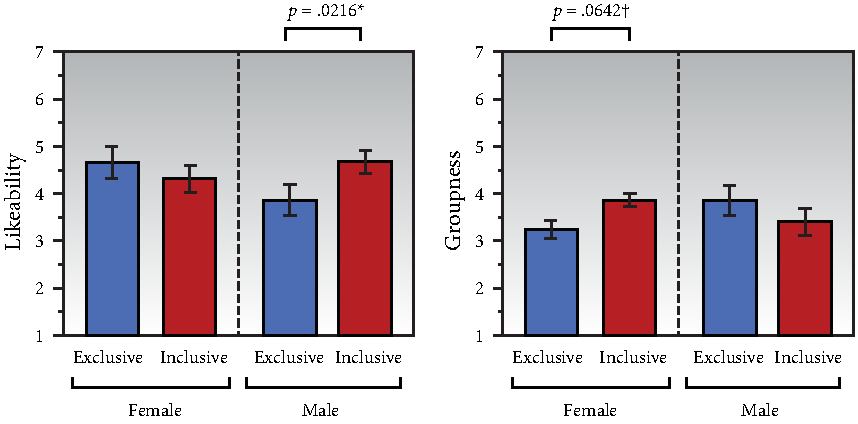
\includegraphics[width=1\textwidth]{conversationalrolegaze/Figures/ResultsSubjectiveGender.pdf}
\caption{Results from two subjective measures (likeability and groupness) by agent behavior (\emph{exclusive} vs. \emph{inclusive}) and participant gender.}
\label{fig:GazeFootingSubjectiveGender}
\end{figure}

Post-hoc analyses revealed a significant, cross-over interaction between agent behavior and participant gender on the \emph{likeability} measure, $F(1, 60) = 5.885, p = .0183$ (Figure~\ref{fig:GazeFootingSubjectiveGender}, left). A pairwise comparison shows that male participants rate the agent exhibiting inclusive behavior significantly higher than when exhibiting exclusive behavior ($F(1, 60) = 5.561, p = .0216$)---this lends partial support to Hypothesis 2. We also found a significant interaction of agent behavior and gender on the \emph{groupness} measure, $F(1, 60) = 4.988, p = .0293$ (Figure~\ref{fig:GazeFootingSubjectiveGender}, right). Female participants assigned marginally higher groupness ratings to the agent exhibiting inclusive behavior than the one displaying exclusive behavior, $F(1, 60) = 3.554, p = .0642$.

\subsection{Discussion}

The experimental results suggest that a virtual agent can use its gaze and body orientation to shape conversational footing of human users (Hypothesis 1) and can do so more effectively in virtual reality (Hypothesis 4). However, there is a comparative lack of evidence that the use of these cues improves users' subjective experiences of the interaction, other than the finding that male participants found the agent more likeable when she looked at them and faced them more (Hypothesis 2), and a marginal improvement in groupness feelings of the female participants in connection with the same manipulation (Hypothesis 6).

The results are not as strong as expected, possibly due to limitations of the system's capabilities and visible agent behavior. One problem that arose during data collection was that the agent would sometimes cut off the participant before they finished their utterance. The lagging of speech recognition results behind the participant's speech production, compounded with the tendency of some participants to pause between utterances, would sometimes cause the system to interpret the lack of incoming speech recognition results as floor release and cut off the participant. This would have had a direct effect on the speaking time measure and might have reduced it substantially in the \emph{inclusive} agent behavior condition.
If the system could have tracked the participants' nonverbal cues during floor-holding pauses (e.g., gaze aversions), it would have been able to avoid such coordination errors.
Furthermore, the effects of the agent's footing cues might have been partially confounded by the more rudimentary aspects of the agent's and confederate's behavior. For example, both the agent and confederate embodiments only had a looping body animation and displayed no body movements connected to the discourse, such as hand gestures. The simplicity of their overall behavior is arguably advantageous from an ecological standpoint, since it places focus onto the agent's gaze, but it could also have seemed unnatural and distracting to participants.

Finally, the interaction effects between the agent's behavior and participant gender were not unexpected.~\citet{mutlu2006storytelling} reported that female participants responded more negatively to increased gaze from a humanlike robot. They linked this result to~\citep{bailenson2001equilibrium}, which found that women tended to maintain greater interpersonal distance than men from a virtual agent displaying increased mutual gaze. Since participants in our experiment had limited control over their position in the scene (they could lean forward and back, but not step away from the agent), high mutual gaze from the agent might have produced negative effects in female participants.
